% !TEX root = presentation.tex
% \begin{frame}
%     \frametitle{Minkowski Sum}
%     \framesubtitle{Example}
%     \topskip0pt
% 	\vspace*{\fill}
%     \begin{center}
%     	\todo[inline]{Schermvullend plaatje}
% 	\end{center}
% 	\vspace*{\fill}
% 	\mbox{\tiny{Image adapted from: \url{http://allenchou.net/2013/12/game-physics-collision-detection-csos-support-functions/}}}
% \end{frame}

\plain{	
	\begin{columns}
		\begin{column}[b]{.25\textwidth}
			\begin{center}
			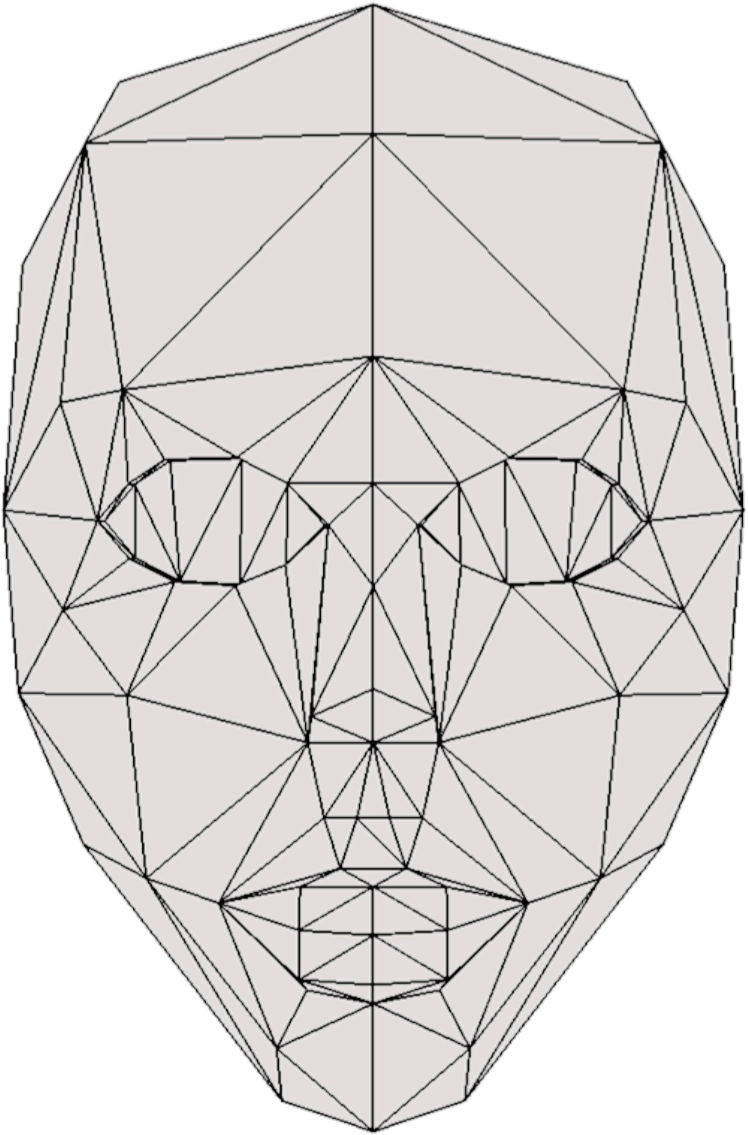
\includegraphics[width=\textwidth]{./img/0_intro/00_results_orange_1.png}
			 \small{input mesh}
			\end{center}
		\end{column}
		\begin{column}[b]{.25\textwidth}
			\begin{center}
			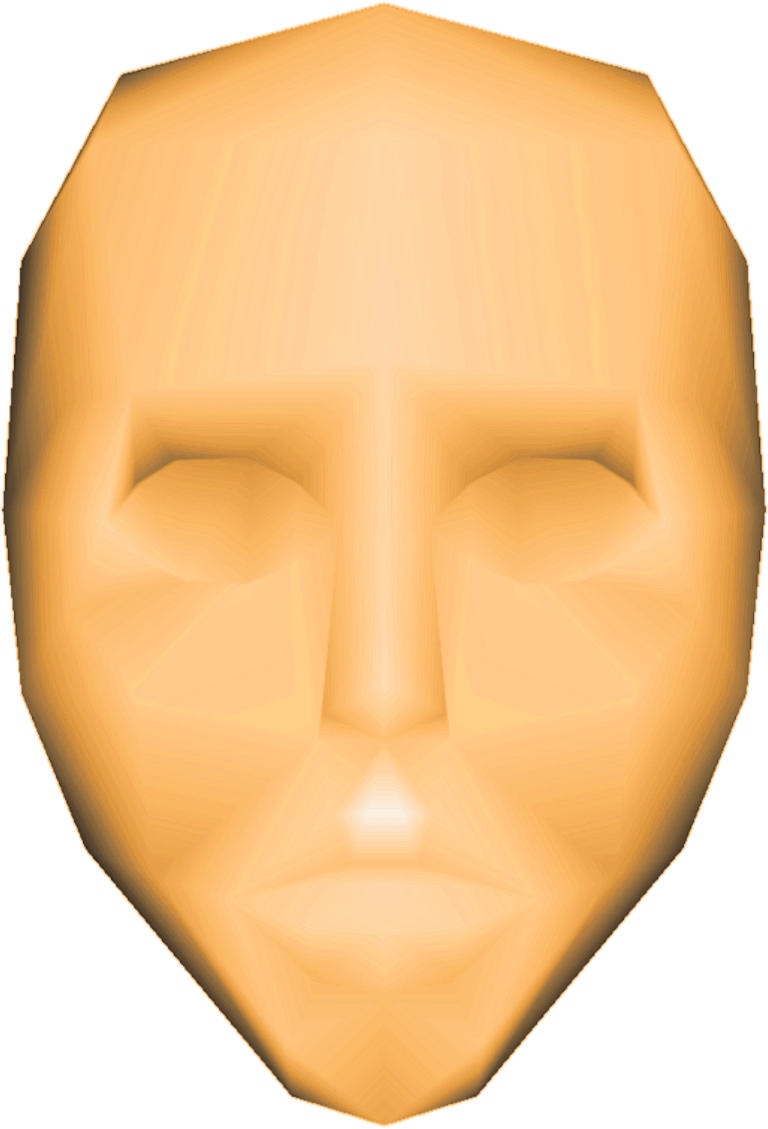
\includegraphics[width=\textwidth]{./img/0_intro/00_results_orange_2.png}
			\small{gouraud}
			\end{center}
		\end{column}
		\begin{column}[b]{.25\textwidth}
			\begin{center}
			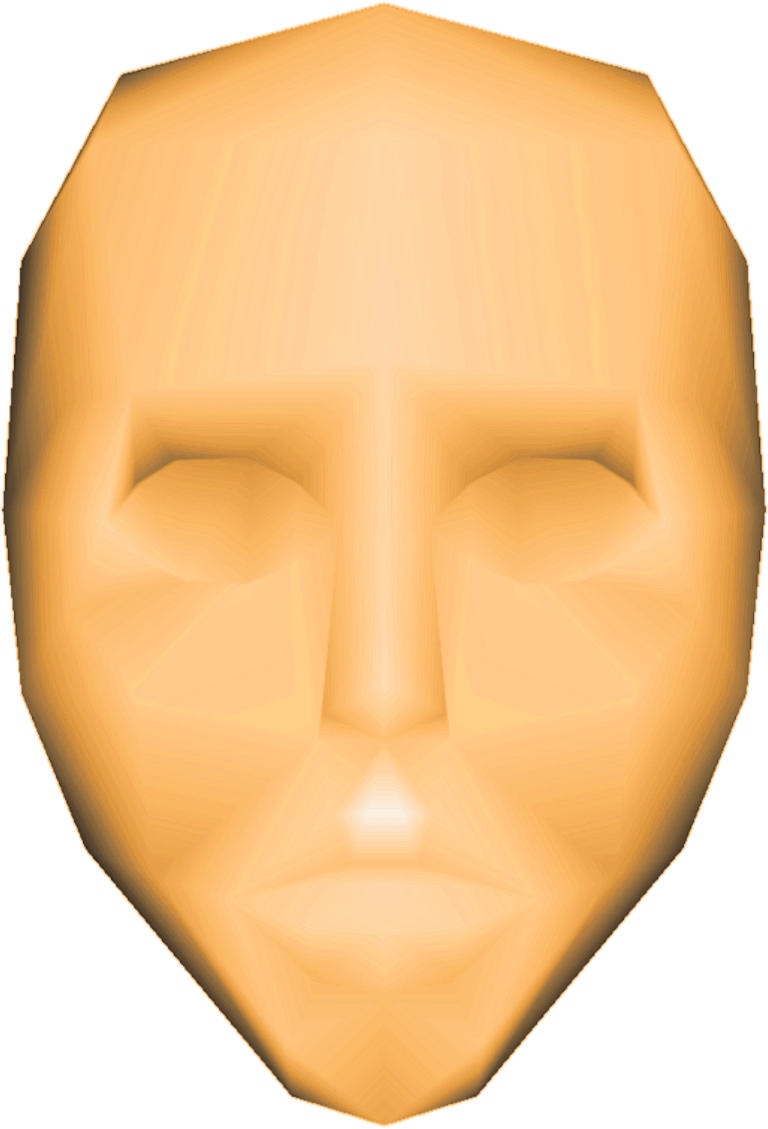
\includegraphics[width=\textwidth]{./img/0_intro/00_results_orange_3.png}
			\small{pn geometry}
			\end{center}
		\end{column}
		\begin{column}[b]{.25\textwidth}
			\begin{center}
			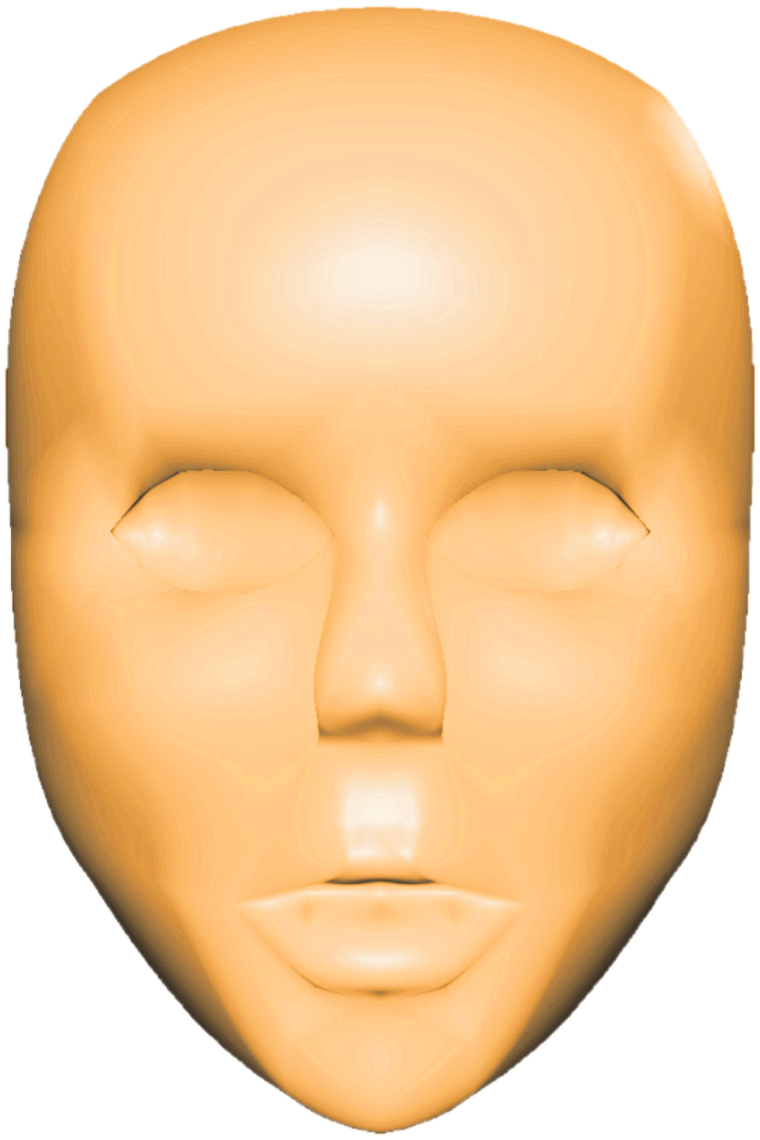
\includegraphics[width=\textwidth]{./img/0_intro/00_results_orange_4.png}
			\small{pn triangles}
			\end{center}
		\end{column}
	\end{columns}
	
	\note{\textbf{[Rick]}}
	\note[item]{Tell what can be seen on the slide.}
	\note[item]{Stand still by the geometry}
	\note[item]{PN triangle -> more \textbf{organic shapes} (and \textbf{continuous surface})}
	\note[item]{Relatively easy to extend existing `pipeline'}
}
